\section{Control por Asignaci\'on de Polos}

Siga los siguientes pasos para sintonizar el controlador mediante asignaci\'on de polos, generar la matriz de ganancias sim\'etrica $K$ y flashear la tarjeta STM32:

\subsection*{Paso 1: Identificaci\'on y Configuraci\'on de Polos Deseados en Julia}
\begin{enumerate}
    \item Abra el archivo \texttt{USER/asignacion\_polos.jl} en el editor.
    \item Ubique el bloque de definici\'on de autovalores o polos deseados en lazo cerrado ($\lambda_1$ a $\lambda_6$).
    \item Asigne las posiciones de los polos asociando cada pareja a su din\'amica f\'isica correspondiente y sus submodos desacoplados:

    \begin{itemize}
        \item $\lambda_{1,2}$: Para controlar la posición y la velocidad lineal.

        \item $\lambda_{3,4}$: Para controlar el angulo y la velocidad angular (cabeceo).
        
        \item $\lambda_{5,6}$: Para controlar el angulo de orientación y velocidad de giro. 
    \end{itemize}
\end{enumerate}

\subsection*{Paso 2: Ejecución, Compilación y Flasheo Autom\'atico}
\begin{enumerate}
    \item Con el archivo \texttt{asignacion\_polos.jl} en pantalla, ejecute el script presionando la combinaci\'on \texttt{Alt + Enter} (o haciendo clic en el bot\'on de Play $\triangleright$ en la esquina superior derecha).
  
    \item Espere a que se realice la compilaci\'on y flasheo de la STM32 y verifique en la consola de Julia la aparici\'on del mensaje de confirmaci\'on indicando la compilaci\'on y flasheo exitoso. Se observar\'a el siguiente mensaje:
\end{enumerate}

\begin{figure}[H]
    \centering
    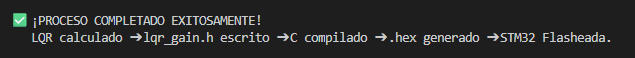
\includegraphics[width=0.7\textwidth]{Images/exito.png}
    \caption{Desarrollo exitoso de la compilaci\'on y flasheo.}
    \label{fig:exito}
\end{figure}

\subsection*{Paso 3: Activaci\'on en el Microcontrolador}
Una vez se haya flasheado la tarjeta STM32 del ROBOT, ubique el mismo sobre una superficie plana libre de obst\'aculos, presione el bot\'on RESET, espere un segundo y presione el bot\'on KEY1.

\subsection*{Paso 4: Ejemplo de Prueba de Referencia (Sintonizaci\'on Inicial)}

Para validar la ejecuci\'on completa del flujo de trabajo y observar una respuesta del sistema estable, configure inicialmente el siguiente conjunto de polos de prueba en \texttt{asignacion\_polos.jl}:

\begin{equation*}
\begin{aligned}
\lambda_{1} &= -50, \quad \lambda_{2} = -10, \\
\lambda_{3} &= -3.5 + 3.5j \quad \lambda_{4} = -3.5 - 3.5j, \\
\lambda_{5} &= -0.5+0.5j, \quad \lambda_{6} = -0.5-0.5j \\
\end{aligned}
\end{equation*}

\begin{enumerate}
    \item Ejecute el script de Julia con la combinaci\'on \texttt{Alt + Enter} o con el bot\'on de tri\'angulo $\triangleright$.
    \item Active el robot presionando el bot\'on RESET, espere un segundo y oprima el bot\'on KEY1 para observar el comportamiento f\'isico.
    \item A partir de las observaciones realizadas con este ejemplo inicial, intente mejorar progresivamente la posici\'on de los polos. \textbf{No lo intente demasiado} más bien pase al control LQR a continuación.
\end{enumerate}




\section{Control LQR}

Siga los siguientes pasos para sintonizar el controlador LQR, generar la matriz de ganancias y flashear la tarjeta STM32.

\subsection*{Paso 1: Identificación y configuración de matrices en Julia}

\begin{enumerate}
	\item Abra el archivo \texttt{USER/control\_lqr.jl} en el editor.
	\item Ubique las matrices de ponderación \texttt{Q\_lqr} ($6 \times 6$) y \texttt{R\_lqr} ($2 \times 2$).
	\item Ingrese los pesos asociando cada posición a su variable física correspondiente:
	
	Matriz de estados $Q_{\text{lqr}}$ ($6 \times 6$):
	\begin{itemize}
		\item \texttt{Q[1,1]}: Posición longitudinal $x$
		\item \texttt{Q[2,2]}: Velocidad longitudinal $\dot{x}$
		\item \texttt{Q[3,3]}: Ángulo de inclinación $\theta$
		\item \texttt{Q[4,4]}: Velocidad angular de inclinación $\dot{\theta}$
		\item \texttt{Q[5,5]}: Ángulo de orientación $\psi$
		\item \texttt{Q[6,6]}: Velocidad angular de giro $\dot{\psi}$
	\end{itemize}
	
	Matriz de control $R_{\text{lqr}}$ ($2 \times 2$):
	\begin{itemize}
		\item \texttt{R[1,1]}: Esfuerzo de control para el motor izquierdo ($u_{\text{izq}}$)
		\item \texttt{R[2,2]}: Esfuerzo de control para el motor derecho ($u_{\text{der}}$)
	\end{itemize}
\end{enumerate}

\subsubsection*{Paso 2: Ejemplo de prueba de referencia (sintonización inicial)}

Para validar la ejecución completa del flujo de trabajo y observar una respuesta del sistema con desempeño limitado, configure inicialmente las siguientes matrices de prueba en \texttt{control\_lqr.jl}:

\begin{verbatim}
	Q_lqr = diagm([2000.0, 0.0, 0.0, 1000.0, 2000.0, 0.0])
	R_lqr = [1.0  0.0;
			0.0  1.0]
\end{verbatim}

\subsubsection*{Paso 3: Generación del archivo de ganancias, compilación y flasheo}

\begin{enumerate}
	\item Con la tarjeta STM32 del robot conectada al computador mediante el cable USB-C y el archivo \texttt{control\_lqr.jl} en pantalla, ejecute el script presionando el atajo \textbf{Alt + Enter} (o haciendo clic en el botón de triángulo $\triangleright$ en la esquina superior derecha).
	\item Espere a que se realice la compilación y el flasheo de la STM32 y verifique en la consola de Julia la aparición del mensaje de confirmación de la Figura~\ref{fig:exito}.
\end{enumerate}

\subsubsection*{Paso 4: Puesta en marcha del robot}

Una vez se haya flasheado la tarjeta STM32 del robot, ubíquelo sobre una superficie plana libre de obstáculos, presione el botón \textbf{RESET}, espere un segundo y presione el botón \textbf{KEY1} (ver la Sección~\ref{sec:encender}).


\section{Asignación}
\begin{enumerate}
	\item A partir de las observaciones realizadas con este ejemplo inicial, reajuste progresivamente las matrices $Q_{\text{lqr}}$ y $R_{\text{lqr}}$ hasta lograr un comportamiento de equilibrio estable y suave y quieto en el punto de equilibrio.
	
	\item Reprograme el robot para que siga una referencia de posición \texttt{ref\_pos}=0.6m. 
	
	\item Reprograme el robot para que siga una referencia de ángulo de orientación  \texttt{ref\_yaw}= $45^o$.
	
	\item Reprograme el robot para que siga una referencia de ángulo de orientación  \texttt{ref\_yaw}= $45^o$ al tiempo que una referencia de posición \texttt{ref\_pos}=0.6m. De ser necesario reajuste los pesos de $Q$ y $R$ como crea conveniente.
\end{enumerate}


